\chapter{Overview}

\pulpino is a single-core System-on-a-Chip built for the \riscv \rvcore and \zerocore core.
\pulpino reuses most components from its bigger brother \pulp.
It uses separate single-port data and instruction RAMs. It includes a boot ROM
that contains a boot loader that can load a program via SPI from an external
flash device.

Figure~\ref{fig:pulpino_overview} shows a block diagram of the SoC.
The SoC uses a AXI as its main interconnect with a bridge to APB for simple
peripherals. Both the AXI and the APB buses feature 32 bit wide data channels.
For debugging purposes the SoC includes an advanced debug unit
which enables access to core registers, the two RAMs and memory-mapped IO via JTAG.
Both RAMs are connected to the AXI bus via bus adapters.

\begin{figure}[H]
  \centering
  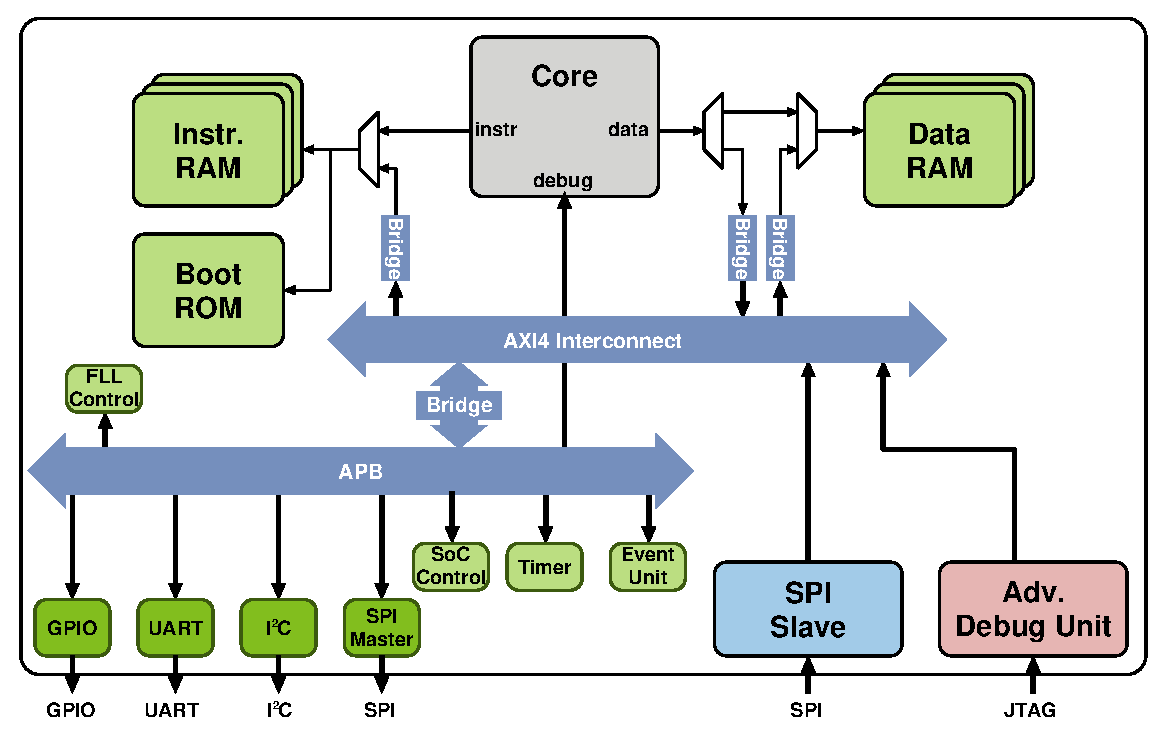
\includegraphics[width=0.9\textwidth]{./figures/pulpino_block.eps}
  \caption{\pulpino Overview.}
  \label{fig:pulpino_overview}
\end{figure}


\pulpino is mainly targeted at RTL simulation and ASICs, although there is also
an FPGA version. The FPGA versions is not specifically optimal in terms of
performance as we mainly use it as a emulation platform rather than a standalone
platform.
